% !TeX root = RJwrapper.tex
\title{A Backbone for Simulating Quantities of Interest from Generalized Linear
Models}
\author{by Christopher Gandrud}

\maketitle

\abstract{%
Simulating quantities of interest estimated from generalized linear
models (GLM) can be an effective way to explore and communicate
statistical results. \pkg{coreSim} provides core functions that can
serve as a reliable and extensible ``backbone'' to new packages for
simulating quantaties of interest for finding and plotting simulated
quantities of interest from GLMs. I demonstrate how to use \pkg{coreSim}
as a backbone by showing how it is incorporated into the new
\pkg{pltesim} package for simulating and displaying probabilistic
long-term effects in models with temporal dependence.
}

\subsection{Introduction}\label{introduction}

There has been a recent trend in the social sciences to improve the
interpretation of results from generalized linear models (GLM) by
presenting estimated quantities of interest from substantively
meaningful scenarios
\citep[e.g.][]{gandrud2005,Licht2011,WilliamsWhitten2012}.
\citet{King2000} advanced a post-estimation simulation technique for
estimating the uncertainty around these estimates. A number of R
packages implement this approach {[}CITE{]}. In particular, the
\CRANpkg{Zelig} package \citep{R-Zelig} implements this technique for a
wide range of model types in an attempt to be ``everyone's statistical
software''.

While all of these packages based on the same simulation procedure, all
of these packages rely on different, custom built ways of doing these
simulations. This presents unnecessarily increases the labor needed to
use post-estimation simulations for showing results in new modelling
situations. Current implementations of these packages have also proven
to be unreliable in ways directly related to their architecture.

In this paper I introduce a new R package--\CRANpkg{coreSim}--that aims
to be an extensible and reliable ``backbone'' for future analyses and R
packages that find post-estimation simulations for substantively
relevant scenarios. I give an example of this by showing how
\pkg{coreSim} forms the basis of the new \pkg{pltesim} package for
simulating and displaying probabilistic long-term effects in models with
temporal dependence.

\subsection{Post-estimation simulations from
GLMs}\label{post-estimation-simulations-from-glms}

One way to estimate substantively meaningful quantities of interest for
complex scenarios from with their associated uncertainty is through
post-estimation
simulations.\footnote{See \citet{King2000} for a comparision with related fully Bayesisan Markov chain Monte Carlo and Bootstrapping methods.}
The procedure is straightforward. Remember that a generalized linear
models can be summarized by two equations. One describes the stochastic
component:

\begin{equation}
Y_{i} \sim f(\theta_{i}, \alpha)
\end{equation}

\noindent Here the dependent variable \(Y\) is a random drawn from the
probability density function \(f(\theta_{i}, \alpha)\). The other
equation describes the systematic component:

\begin{equation}
\theta_{i} = g(X_{i}, \beta),
\end{equation}

where \(X\) is a vector of explanatory variables and \(\beta\) is a
vector of effect parameters. The function \(g\) is often referred to as
the link function, which specifies how the variables and effect
parameters are translated into \(\theta\).

We can use post-estimation simulations to find and communicate
substantively meaningful results from these models. To do this we first
estimate \(\hat{\beta}\) and \(\hat{\alpha}\). Second, we drawn \(n\)
number of values of these parameters from the multivariate normal
distribution using the parameter point estimates and their variance
covariance matrix with a mean of \(\hat{\gamma}\)--a vector created by
stacking \(\hat{\beta}\) and \(\hat{\alpha}\)--and variance of
\(\hat{\mathrm{V}}(\hat{\gamma})\):

\begin{equation}
\widetilde{\gamma} \sim \mathrm{N}(\hat{\gamma}, \hat{\mathrm{V}}(\hat{\gamma})) 
\end{equation}

Drawing these simulations is straightforward using two functions from
the \CRANpkg{stats} package--\code{coef} and \code{vcov}--as well as the
\code{mvrnorm} function from the \CRANpkg{MASS} package. Both
\CRANpkg{stats} and \CRANpkg{MASS} are included with the default R
installation. For example:

\begin{Schunk}
\begin{Sinput}
# Load package that contains the Prestige data set
library(car)

library(MASS)

# Estimate normal linear model
m1 <- lm(prestige ~ education + type, data = Prestige)

# Extract coeficient estimates
m1_coef <- coef(m1)

# Extract variance-covariance matrix
m1_vcov <- vcov(m1)

# Draw 1000 simulations from multivariate normal distribution
m1_sims <- mvrnorm(n = 1000, mu = m1_coef, Sigma = m1_vcov)

head(m1_sims)
\end{Sinput}
\begin{Soutput}
#>       (Intercept) education  typeprof      typewc
#> [1,]  -2.46299473  4.479084  6.791089  -1.1362359
#> [2,]  -3.37548512  4.822845  1.722389  -6.1467418
#> [3,]  -9.23523872  5.116772  7.931571  -4.9137734
#> [4,] -10.82754562  5.565439 -2.061336 -10.0247785
#> [5,]  -0.06587696  3.996145 10.140270  -0.5249211
#> [6,]   4.38447086  3.891146  7.054453  -5.1137317
\end{Soutput}
\end{Schunk}

Now that we have the simulated effect coefficients, we can find our
quantity of interest for a given scenario. In this example, our quantity
of interest is simply the predicted value of the \code{prestige}
dependent variable. We simply need to find the systematic component from
the linear form for each simulation:
\(g(X_{i}, \beta) = X_{i}\beta_{i} = \beta_{0} + X_{i1}\beta_{1} + X_{i2}\beta_{2} + \ldots\).
For example imagine that we want to find the predicted level of
\code{prestige} when \code{education} is at its median (10.54) and the
type of profession is \code{prof}. We could calculate \code{prestige}
for this scenario using:

\begin{Schunk}
\begin{Sinput}
# Create a data frame with the scenario values
fitted <- data.matrix(data.frame(education = 10.54, typeprof = 1))

# Reformat simulations
intercept <- m1_sims[, 1] # extract intercept
other_betas <- data.matrix(m1_sims[, colnames(fitted)]) 

# Find quantitiy of interest
qi <- intercept + (other_betas %*% c(fitted))

head(qi)
\end{Sinput}
\begin{Soutput}
#>          [,1]
#> [1,] 51.53764
#> [2,] 49.17970
#> [3,] 52.62711
#> [4,] 45.77085
#> [5,] 52.19376
#> [6,] 52.45161
\end{Soutput}
\end{Schunk}

Finally, we can trim of outliers by keeping the central 95\% interval
and then visualise the results.

\begin{Schunk}
\begin{Sinput}
# Find lower and upper bound of the simulations' central 95% interval 
lower_bound <- quantile(qi, probs = 0.25)
upper_bound <- quantile(qi, probs = 0.975)

# Restrict the simulations to the central 95% interval
qi <- qi[qi > lower_bound]
qi <- qi[qi < upper_bound]

# Plot
plot(density(qi))
\end{Sinput}

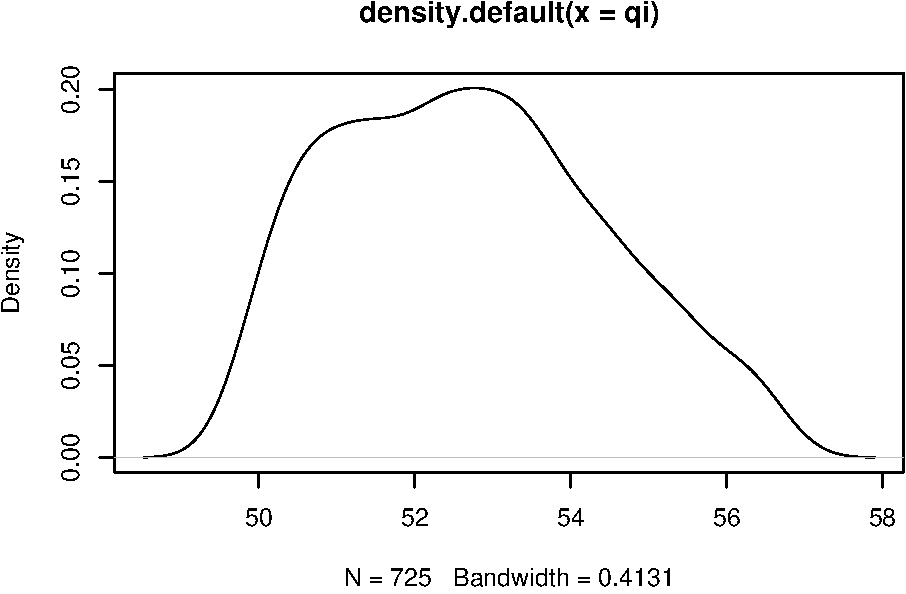
\includegraphics{gandrud_files/figure-latex/unnamed-chunk-3-1} \end{Schunk}

This is a trivial example that shows the basic steps required to find
quantities of interest from post-estimation simulations. The use of this
technique in this context does not provide us with much more information
than we could relatively easily find using the point estimates
themselves and their confidence intervals. Where post-estimation
simulations are much more useful is for exploring more complex,
contrasting scenarios, often with interactions and non-linearities.
These relationships can be difficult to meaningfully interpret with
individual point estimates and their associated confidence intervals.

The process for finding these scenarios with post-estimation simulations
is in practice much more difficult as it requires calculating quantities
of interest for each scenario.

\subsection{Previous post-estimation simulation
packages}\label{previous-post-estimation-simulation-packages}

The \CRANpkg{Zelig} package could potentially help streamline this
process and in so doing form the basis of R packages that generate
post-estimation simuliations in novel areas.

\CRANpkg{Zelig} has a number of issues that have made it unreliable over
time. By aiming to be everyone's statistical software, \CRANpkg{Zelig}
relies on many (13 imported) dependencies.

\subsection{Summary}\label{summary}

\bibliography{gandrud}

\address{%
Christopher Gandrud\\
City University London and Hertie School of Governance\\
Rhind Building\\ London, EC1V 0HB\\
}
\href{mailto:christopher.gandrud@city.ac.uk}{\nolinkurl{christopher.gandrud@city.ac.uk}}

